\selectlanguage{ngerman}%
\frenchspacing%
\begin{ledgroupsized}[r]{120mm}%
\footnotesize%
\pstart%
\noindent\textbf{Überlieferung:}%
\pend%
\end{ledgroupsized}%
\begin{ledgroupsized}[r]{114mm}%
\footnotesize%
\pstart%
\parindent -6mm%
\makebox[6mm][l]{\textit{L}}%
Aufzeichnung:
LH~XXXVII~3 Bl.\:125\textendash127.
Ein Bogen 2\textsuperscript{o}\! (Bl.\:125\textendash126) und ein Einzelblatt~2\textsuperscript{o}\! (Bl.\:127);
Wasserzeichen auf Bl.\:\href{\Scan{LH_37_03_125wz}}{125};
unterer Rand von Bl.\:\href{\Scan{LH_37_03_127r}}{127\:r\textsuperscript{o}}\! ausgefranst mit geringfügigem Textverlust 
(der verlorene Text ist in dem 1967 aufgenommenen S-Film Nr.\:116 der GWLB Hannover noch lesbar):
Papiererhaltungsmaßnahmen.
Fünfeinhalb Seiten einspaltig beschrieben;
untere Hälfte von Bl.\:\href{\Scan{LH_37_03_127v}}{127\:v\textsuperscript{o}}\! unbeschrieben.
Textfolge nach Blattzählung;
ein Kustos am Ende von Bl.\:\href{\Scan{LH_37_03_126v}}{126\:v\textsuperscript{o}}\! verweist auf den Anfang von Bl.\:\href{\Scan{LH_37_03_127r}}{127\:r\textsuperscript{o}}.
\pend%
\end{ledgroupsized}%
\vspace{5mm}%
\begin{ledgroup}%
\footnotesize%
\pstart%
\noindent%
\textbf{Datierungsgründe:}
Die Datierung der Aufzeichnung N.\;\ref{60212} beruht auf äußeren Eigenschaften des Text\-trägers %
sowie auf inhaltlichen Betrachtungen.
Siehe die ausführliche Begründung auf S.\;\pageref{60212_dat}.
\pend%
\end{ledgroup}%
\selectlanguage{latin}%
\frenchspacing%
\vspace{8mm}%
\normalsize%
\pstart%
\noindent%
\lbrack%
\href{\Scan{LH_37_03_125r}}%
{125\:r\textsuperscript{o}}%
\rbrack%
\pend%
\begin{edfigure}[0.750em][0.000em]%
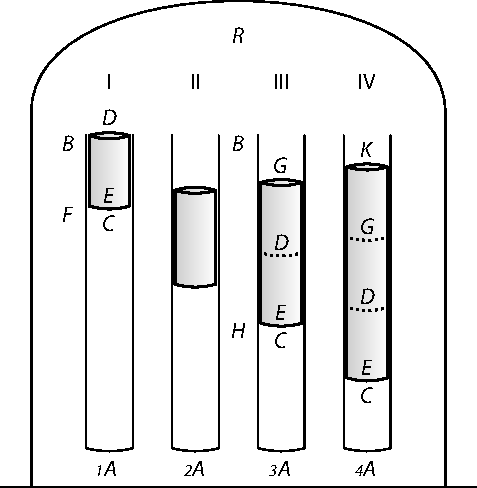
\includegraphics[width=0.64\textwidth]{gesamttex/edit_VIII-4/images/LH_37_03_125-127_d1_125r.pdf}%
\edcaption[1.0em]{%
\lbrack\textit{Fig.\:1}\rbrack%
}%
\end{edfigure}%
\newpage%
\pstart%
\edtext{%
(1)%
}{%
\lemma{(1)}%
\Bfootnote{%
\textit{erg.\:L}}}
Aer est corpus grave fluidum elasticum.%
\indexS{aer corpus grave fluidum elasticum}%
\indexS{corpus grave}%
\indexS{corpus fluidum}%
\indexS{corpus elasticum}
\pend%
\pstart%
\edtext{%
(2)%
}{%
\lemma{(2)}%
\Bfootnote{%
\textit{erg.\:L}}}%
\textls{ Corpus elasticum }%
\indexS{corpus elasticum}%
voco
quod
vi quadam externa adhibita%
\indexS{vis externa}%
\indexS{vis adhibita}
figuram suam aut volumen mutat,%
\indexS{figura corporis elastici}%
\indexS{volumen corporis elastici}
eaque vi amota%
\indexS{vis amota}
ad
\edtext{%
eam redit.%
}{%
\lemma{eam}%
\Bfootnote{%
\textit{(1)}~reditur. %
\textit{(2)}~redit.%
~\textit{L}%
}}
Vim autem ipsius corporis%
\indexS{vis corporis elastici}
qua externo
\edtext{%
innit\lbrack e\rbrack nti%
}{%
\lemma{innitanti}%
\Bfootnote{%
\textit{L~ändert Hrsg.}%
}}
renititur%
\indexS{vis externa}%
\indexS{vis innitens}%
\indexS{vis renitens}
et ad statum%
\indexS{status prior}%
\indexS{vis tendens ad statum priorem}
\edtext{%
suum priorem tendit,%
}{%
\lemma{suum}%
\Bfootnote{%
\textit{(1)}~te %
\textit{(2)}~redit, %
\textit{(3)}~priorem tendit,%
~\textit{L}%
}}
voco\textls{ Elastrum.}%
\indexS{elastrum}
\pend%
\pstart%
\edlabel{LH_37_03_125-127_127r_axioma-1}%
\edtext{(3)}{%
\lemma{(3)}\Bfootnote{%
\textit{erg.\;L}}}
Effectus sunt causis proportionales,%
\indexS{effectus proportionalis causae}%
\indexS{causa proportionalis effectui}
vel ut distinctius exponam,
\edtext{%
si in idem%
}{%
\lemma{si}%
\Bfootnote{%
\bars{in \textit{erg.}}
idem%
~\textit{L}%
}}
patiens%
\indexS{patiens}
in eodem statu
\edtext{%
positum %
agat vel \textit{A} vel \textit{B},
sitque agens integrum \textit{A}%
\indexS{agens integrum}%
\indexS{agentia similia}
agenti integro \textit{B} simile,%
}{%
\lemma{positum}\Bfootnote{%
\textit{(1)}~sit, et int %
\textit{(2)}~agat vel %
\bars{agens \textit{gestr.}} %
\textit{A} vel %
\bars{agens \textit{gestr.}} %
\textit{B}, sitque agens integrum \textit{A} %
\textit{(a)}~simile %
\textit{(b)}~agenti integro \textit{B} simile,%
~\textit{L}%
}}
saltem quatenus agunt,
erunt etiam effectus similes,%
\indexS{effectus similis agenti}
seu agentibus%
\indexS{effectus proportionalis agenti}
\edlabel{LH_37_03_125-127_125r_ibwr-1}%
proportionales.%
\edlabel{LH_37_03_125-127_127r_axioma-2}
\edtext{}{%
\xxref{LH_37_03_125-127_125r_ibwr-1}{LH_37_03_125-127_125r_ibwr-2}%
\lemma{proportionales.}%
\Bfootnote{%
\textit{(1)}~Si %
\textit{(a)}~eni %
\textit{(b)}~ex %
\textit{(2)}~Ut %
\textit{(3)}~\lbrack/\rbrack\ (4) Hinc si %
\bars{idem \textit{erg.}} %
patiens%
~\textit{L}%
}}%
\pend%
\pstart%
(4)
Hinc si idem patiens%
\indexS{patiens}%
\edlabel{LH_37_03_125-127_125r_ibwr-2}
\edtext{%
prematur duobus diversis ponderibus%
\indexS{pondus premens}
libere ab aliquo filo suspensis,%
\indexS{pondus suspensum a filo}
tunc utique%
}{%
\lemma{prematur}%
\Bfootnote{%
\textit{(1)}~nunc pondere %
\bars{libere suspenso \textit{erg.}} \textit{A} %
\textit{(2)}~nunc pondere %
\textit{(a)}~\textit{B} %
\textit{(b)}~libere suspenso %
\textit{(c)}~uno, nunc altero %
\textit{(d)}~\textit{A} nunc pondere \textit{B} (quae pondera ambo libere agere suppono)%
\indexS{pondus agens libere} %
\textit{(3)}~duobus diversis %
\lbrack...\rbrack\ tunc utique%
~\textit{L}%
}}
cum
\edtext{%
non ipsius figurae corporum%
\indexS{figura corporis}
aut alterius circumstantiae,%
\indexS{circumstantia alia}
sed gravitatum%
\indexS{gravitas}
tantummodo ratio habeatur,%
}{%
\lemma{non}%
\Bfootnote{%
\textit{(1)}~figur\textlangle a\textrangle\ %
\textit{(2)}~ipsisus figurae corporum %
\textit{(a)}~aliarumque circumstatiarum %
\textit{(b)}~aut alterius circumstantiae, sed %
\textit{(aa)}~solarum %
\textit{(bb)}~gravitatum tantummodo ratio habeatur,%
~\textit{L}%
}}
patet
\edtext{%
ipsos%
}{%
\lemma{ipsos}%
\Bfootnote{\textit{erg.\;L}%
}}
effectus%
\indexS{effectus pressionis}
qui ex illa pressione sequuntur%
\indexS{pressio}
fore ponderibus proportionales.%
\indexS{effectus proportionalis ponderi}
Duo enim pondera,
per se spectata,%
\indexS{pondus spectatum per se}
sunt agentia similia,%
\indexS{agentia similia}
\edtext{%
quia in ipsis solam quantitatem gravitatis spectamus;%
\indexS{quantitas gravitatis}%
\indexS{gravitas}
similia autem vocantur,
quae sola quantitate discernimus.%
\indexS{discretum sola quantitate}%
}{%
\lemma{quia}%
\Bfootnote{%
\textit{(1)}~simile %
\textit{(2)}~similia vocamus quae non p %
\textit{(3)}~in ipsis solam quantitatem %
\textit{(a)}~ponderis %
\textit{(b)}~gravitatis spectamus; %
\lbrack...\rbrack\ quantitate discernimus.%
~\textit{L}%
}}
\pend%
\pstart%
(5)
Sit jam
\edtext{%
tubus%
\indexS{tubus cylindricus}
\edtext{cylindricus}{%
\lemma{cylindricus}%
\Bfootnote{\textit{erg.\;L}%
}}
\textit{AB}%
}{%
\lemma{tubus cylindricus \textit{AB}}%
\Cfootnote{%
Vgl. das Diagramm \lbrack\textit{Fig.\:1}\rbrack.%
}}
positus in
\edtext{Recipiente}{%
\lemma{Recipiente}%
\Bfootnote{\textit{erg.\;L}%
}}
Vacuo \textit{R}.%
\indexS{recipiens vacuus}
\edtext{%
Vacuum autem intelligo Gerickianum,%
\indexN{\textls{Guericke} (Gerickius, Gericke), Otto von 1602\textendash1686}%
\indexS{vacuum Gerickianum}%
}{%
\lemma{Vacuum \lbrack...\rbrack\ Gerickianum}%
\Cfootnote{%
Siehe %
O.\;v.\;\textsc{Gue\-ri\-cke}, \textit{Experimenta nova}, l.\;II, cap.\;3 (Amsterdam 1672, S.\;56a).\cite{00055}
Guerickes Versuche über das Vakuum werden ebd., l.\;III (S.\;71\,ff.) dargestellt.
Leibnizens Auszüge hieraus %
sind in \textit{LSB} VIII,\;1 N.\;36\cite{01197} ediert.%
}}
in quo aer aut nullus aut exiguus%
\indexS{aer nullus in recipiente}%
\indexS{aer exiguus in recipiente}
\edtext{%
restat%
\lbrack,
i\rbrack n
ipso%
}{%
\lemma{restat.}%
\Bfootnote{%
In
\textit{L\;ändert Hrsg.}%
}}
scilicet recipiente:%
\indexS{recipiens vacuus}
in Tubo autem sit aer \textit{AC}%
\indexS{tubus cylindricus}
pondere%
\indexS{pondus comprimens aerem}
\edtext{%
corporis \textit{DE}
(Hydrargyri%
\indexS{hydrargyros}
si placet)%
}{%
\lemma{corporis}%
\Bfootnote{%
\textit{(1)}~\textit{BC} %
\textit{(2)}~\textit{DE} %
\textit{(a)}~quod %
\textit{(b)}~(Hydrargyri si placet)%
~\textit{L}%
}}
compressus%
\indexS{aer compressus}
et in tubi parte \textit{AC} retentus,%
\indexS{aer retentus in tubo}
quominus inde exire%
\indexS{aer exiens}
et in naturalem magis Statum%
\indexS{status naturalis}
se dilatare possit.%
\indexS{aer dilatans se in statum naturalem}
\edlabel{LH_37_03_125-127_125r_sdfi-1}%
Patet Elastrum huius aeris%
\indexS{elastrum aeris compressi}
\edtext{%
\textit{AC}%
}{%
\lemma{\textit{AC}}%
\Bfootnote{\textit{erg.\;L}%
}}
(seu vim se dilatandi)%
\indexS{vis aeris dilatandi}
tantum esse
quantum
\edtext{%
est pondus \textit{DE}.%
\indexS{pondus comprimens aerem}
}{%
\lemma{est pondus}%
\Bfootnote{%
\textit{(1)}~\textit{BC}. %
\textit{(2)}~\textit{DE}.%
~\textit{L}%
}}
Sunt enim inter se in aequilibrio nisus%
\indexS{nisus in aequilibrio}
(ex hypothesi)%
\indexS{hypothesis}
neque aut pondus descendere%
\indexS{pondus descendens}
aut aer se dilatare amplius potest,%
\indexS{aer dilatans se}
altero alterum impediente.%
\edlabel{LH_37_03_125-127_125r_sdfi-2}
\edtext{%
Cum enim res in vacuo geri ponatur,%
\indexS{res gesta in vacuo}%
\indexS{vacuum}
nihil aliud est %
quod ad hunc effectum contribuat,%
\indexS{effectus compressionis}
cum alioqui aeris ambientis et incumbentis%
\indexS{aer ambiens}%
\indexS{aer incumbens}
quoque ratio habenda fuisset.%
}{%
\lemma{}\Bfootnote{%
Cum enim \lbrack...\rbrack\ habenda fuisset.
\textit{erg.\;L}%
}}
\pend%
\pstart%
(6)
Ponamus jam pondus comprimens augeri,%
\indexS{pondus comprimens aerem}%
\indexS{pondus auctum}%
\indexS{pondus duplum}
seu fieri duplo majus,
\edtext{%
sive ipsi Mercurio \textit{DE}%
\indexS{mercurius infusus}%
}{%
\lemma{sive}%
\Bfootnote{%
\bars{ipsi \textit{erg.}} Mercurio %
\textit{(1)}~\textit{BC} %
\textit{(2)}~\textit{DE}%
~\textit{L}%
}}
tantundem adhuc affundi%
\lbrack,\rbrack\
\edtext{%
nempe \textit{GD}.%
}{%
\lemma{nempe \textit{GD}}%
\Bfootnote{\textit{erg.\;L}%
}}
Quaeritur%
\lbrack:\rbrack\
\lbrack%
\href{\Scan{LH_37_03_125v}}%
{125\:v\textsuperscript{o}}%
\rbrack\
Quanta futura sit aeris tubo inclusi compressio?%
\indexS{aer inclusus tubo}%
\indexS{aer compressus in tubo}%
\indexS{compressio aeris}
Respondeo
dubium nullum esse,
quin compressio futura sit dupla prioris.%
\indexS{compressio dupla}
Vis enim dupla per omnia similis similiterque agens,%
\indexS{vis dupla}%
\indexS{vis similis}%
\indexS{vis agens similiter}
utique effectum etiam duplum dabit,%
\indexS{effectus duplus}
per axioma%
\indexS{axioma}
positum articulo%
\indexS{articulus}
\edtext{%
\lbrack tertio\rbrack.%
}{%
\lemma{secundo}\Bfootnote{%
\textit{L~ändert Hrsg.}%
}%
\lemma{\lbrack tertio\rbrack}%
\Cfootnote{%
Vgl. \refpassage{LH_37_03_125-127_127r_axioma-1}{LH_37_03_125-127_127r_axioma-2}.%
}%
}%
\pend%
\pstart%
(7)
Compressio autem%
\indexS{compressio aeris}%
\indexS{aer compressus in tubo}
\edtext{%
aeris \textit{AC}%
}{%
\lemma{aeris \textit{AC}}%
\Cfootnote{%
Vgl. das Diagramm \lbrack\textit{Fig.\:2}\rbrack.%
}}
cum per se non possit aestimari nec cognosci%
\indexS{compressio aestimata}%
\indexS{aestimatio compressionis}
nisi ex spatio
intra quod per vim redigitur,%
\indexS{spatium intra quod aer comprimitur}%
\indexS{vis compressionis}
\edtext{%
ideo
cum aer \textit{AC} antea in Tubo \textit{AB}
(sub num.\;I posito\lbrack)\rbrack\
compressus sit a pondere \textit{DE}%
\indexS{pondus comprimens aerem}
intra spatium \textit{AF},
utique nunc aucto pondere \textit{GDE},%
\indexS{pondus auctum}
idem aer \textit{AC}
in Tubo eodem \textit{AB}%
\indexS{tubus cylindricus}
(sub num.\;II posito%
\lbrack)\rbrack\
comprimetur in spatium arctius \textit{AH}.%
\indexS{aer compressus in tubo}
}{%
\lemma{ideo}%
\Bfootnote{%
\textit{(1)}~proximum est ut dicamus, %
\textit{(2)}~cum aer %
\lbrack...\rbrack\ (sub num.\;I %
\bars{) posito \textit{ändert Hrsg.}} compressus %
\bars{sit \textit{erg.}} a pondere \textit{DE} intra spatium %
\textit{(a)}~\textit{AC} %
\textit{(b)}~\textit{AF}, %
\textit{(aa)}~et nunc duplic %
\textit{(bb)}~utique nunc %
\textit{(aaa)}~duplicato %
\textit{(bbb)}~aucto pondere \textit{GDE}, %
\textit{(aaaa)}~com %
\textit{(bbbb)}~idem aer %
\lbrack...\rbrack\ eodem \textit{AB} %
\textit{(aaaaa)}~posito %
\textit{(bbbbb)}~(sub num.\;II %
\bars{) posito \textit{ändert Hrsg.}} %
comprimetur in spatium arctius \textit{AH}.%
~\textit{L}%
}}
\pend%
\pstart%
\edlabel{LH_37_03_125-127_125v_fgso-1}%
(8)
Quaeritur jam
quantum esse debeat spatium \textit{AH}.%
\indexS{spatium in quod aer redigitur}
Seu data ratione ponderis \textit{GDE} ad pondus \textit{DE},%
\indexS{ratio ponderum dupla}
\edtext{%
quae in hoc casu est dupla,%
}{%
\lemma{quae}%
\Bfootnote{%
\textit{(1)}~hoc loco est %
\textit{(2)}~in hoc casu est dupla,%
~\textit{L}%
}}
quaeritur
quae sit ratio spatii%
\indexS{ratio spatiorum subdupla}
\edtext{%
\textit{AH}
sub pondere \textit{GDE}%
}{%
\lemma{\textit{AH}}%
\Bfootnote{%
\textit{(1)}~(\textlangle a\textrangle\ pondere \textit{GDE} %
\textit{(2)}~sub pondere \textit{GDE}%
~\textit{L}%
}}
ad spatium \textit{AF}
sub
\edtext{%
pondere \textit{DE}.%
}{%
\lemma{pondere}%
\Bfootnote{%
\textit{(1)}~\textit{A} %
\textit{(2)}~\textit{DE} %
\textit{(3)}~\textit{DE}%
~\textit{L}%
}}
Respondeo
eam esse subduplam,%
\indexS{ratio spatiorum subdupla}
sive \textit{AH} esse dimidium ipsius \textit{AF};
si vero pondus \textit{KGDE}
\edtext{sub numero III%
}{%
\lemma{sub numero III}%
\Bfootnote{%
\textit{erg.\;L}%
}}
esset triplum ponderis%
\indexS{pondus comprimens aerem}%
\indexS{ratio ponderum tripla}
\edtext{%
\textit{DE},
tunc spatium \textit{AL}
for\lbrack e\rbrack\
subtriplum%
}{%
\lemma{\textit{DE},}%
\Bfootnote{%
\bars{tunc \textit{erg.}} spatium %
\textit{(1)}~\textit{AH} %
\textit{(2)}~\textit{AL} %
\bars{foret \textit{ändert Hrsg.}} %
subtriplum%
~\textit{L}%
}}
seu tertia pars spatii \textit{AF};%
\indexS{ratio spatiorum subtripla}
et generaliter
\edtext{%
spatia
intra quae corpus elasticum comprimitur%
\indexS{spatium intra quod aer comprimitur}
fore in ratione reciproca ponderum comprimentium,%
\indexS{spatia in ratione reciproca ponderum comprimentium}%
\indexS{pondus comprimens aerem}
sive%
}{%
\lemma{}%
\Bfootnote{%
spatia intra \lbrack...\rbrack\ comprimentium, sive
\textit{erg.\;L}%
}}
spatium%
\indexS{spatium intra quod aer comprimitur}
\edtext{%
}{%
\xxref{LH_37_03_125-127_125v_hfkd-1}{LH_37_03_125-127_125v_hfkd-2}%
\lemma{\textit{AH}}%
\Bfootnote{%
\bars{sub pondere \textit{DEG} \textit{erg. u. gestr.}}
fore ad spatium \textit{AF}
\textit{(1)}~in ratione ponderum %
\textit{(2)}~sub pondere \textit{AF} %
\textit{(3)}~sub pondere %
\textit{(4)}~in ratione ponderis \textit{A} %
\textit{(5)}~ut est pondus %
\textit{(a)}~\textit{DE} %
\textit{(b)}~\textit{DE} %
\textit{(c)}~\textit{ED} %
\textit{(d)}~\textit{DE}, sub quo %
\lbrack...\rbrack\ pondus \textit{GDE} %
\textit{(aa)}~sub quo est spatium \textit{AH}. Id quod %
\textit{(bb)}~sub quo %
\lbrack...\rbrack\ est, quod%
~\textit{L}%
}}%
\edlabel{LH_37_03_125-127_125v_hfkd-1}%
\textit{AH} fore ad spatium \textit{AF}
ut est pondus \textit{DE},
sub quo est spatium \textit{AF},
ad pondus \textit{GDE},%
\indexS{pondus comprimens aerem}
sub quo est spatium \textit{AH}.%
\indexS{spatium intra quod aer comprimitur}%
\indexS{spatia in ratione reciproca ponderum comprimentium}%
\edlabel{LH_37_03_125-127_125v_fgso-2}
\pend%
\pstart%
(9)
Id autem ex eo manifestum est,
quod%
\edlabel{LH_37_03_125-127_125v_hfkd-2}%
\textls{ }%
\edlabel{LH_37_03_125-127_125v_thnd-1}%
\textls{spatia sunt in reciproca ratione compressionum,}%
\indexS{spatia in ratione reciproca compressionum}%
\edlabel{LH_37_03_125-127_125v_thnd-2}
\edtext{%
sive,
si aer \textit{AC} intra spatium \textit{AH}
sit duplo (triplo) compressior%
\indexS{aer compressior duplo}%
\indexS{aer compressior triplo}
quam idem aer \textit{AC}%
\indexS{aer compressus in tubo}
intra spatium \textit{AF},%
\indexS{spatium intra quod aer comprimitur}%
}{%
\lemma{sive,}%
\Bfootnote{%
\textit{(1)}~si aer sit duplo %
\textit{(2)}~si aer \textit{AC} %
\textit{(a)}~sit duplo compressior aere \textit{A} %
\textit{(b)}~intra spatium \textit{AH} sit duplo %
\bars{(triplo) \textit{erg.}} %
compressior quam %
\lbrack...\rbrack\ spatium \textit{AF},%
~\textit{L}%
}}
\edlabel{LH_37_03_125-127_125v-126r_vdvd-1}%
\edtext{%
}{%
\xxref{LH_37_03_125-127_125v-126r_vdvd-1}{LH_37_03_125-127_125v-126r_vdvd-2}%
\lemma{utique intra spatium}%
\Bfootnote{%
\bars{\textit{AH} \textit{erg.}} duplo %
\textit{(1)}~vel %
\textit{(2)}~(triplo) %
\textit{(a)}~minus, sive %
\textit{(b)}~arct %
\textit{(c)}~angustius, sive subduplum (subtriplum) %
\textit{(aa)}~compressus erit %
\textit{(bb)}~prioris spatii \textit{AF}, compressus erit. %
\textit{(aaa)}~Suppono enim velut principium totius tractationis hujus de Elastro, vim a%
\indexS{elastrum aeris}\indexS{tractatio de elastro} %
\textit{(bbb)}~Suppono %
\textit{(ccc)}~Hanc ipsam %
\lbrack...\rbrack\ \textls{compressionem} appello. %
\bars{\lbrack/\rbrack\ (10) \textls{Compressiones autem} %
\lbrack...\rbrack\ se liberare. \textit{erg.}} Aerem enim %
\lbrack...\rbrack\ homogenei %
\href{\Scan{LH_37_03_126r}}{\lbrack126\:r\textsuperscript{o}\rbrack} considero,%
~\textit{L}%
}}%
utique intra spatium \textit{AH}%
\indexS{spatium intra quod aer comprimitur}
duplo (triplo) angustius,%
\indexS{spatium duplo angustius}%
\indexS{spatium triplo angustius}
sive subduplum (subtriplum) prioris spatii \textit{AF},
compressus erit.%
\indexS{aer compressus in tubo}%
\indexS{spatia in ratione reciproca compressionum}
Hanc ipsam enim angustiae quantitatem%
\textls{ compressionem }appello.%
\indexS{quantitas angustiae}%
\indexS{compressio ut quantitas angustiae}%
\indexS{compressio aeris}
\pend%
\begin{edfigure}[2.50em][0.00em]%
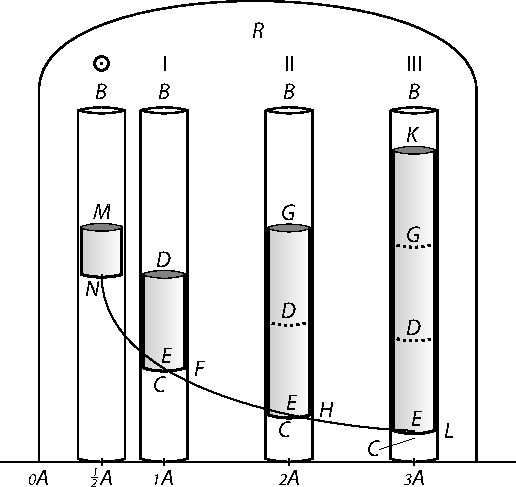
\includegraphics[width=0.61\textwidth]{gesamttex/edit_VIII-4/images/LH_37_03_125-127_d2_125v.pdf}%
\edcaption[0.75em]{%
\edtext{%
\lbrack\textit{Fig.\:2}\rbrack%
}{%
\lemma{\textit{Über dem Diagramm} \lbrack\textit{Fig.\:2}\rbrack:}%
\Afootnote[nonum]{%
$%
\quad\quad%
\displaystyle%
\frac{1}{2}
\quad\quad%
1%
\quad\quad%
1%
$%
\newline%
\hspace*{48.5mm}%
$%
\displaystyle%
\frac{1}{2}%
\quad\quad%
1%
\quad\quad%
2%
\quad\quad%
3%
$%
\newline%
\hspace*{49.5mm}%
$%
\displaystyle%
2%
\quad\quad%
\hspace*{0.4mm}%
1%
\quad\quad%
\hspace*{-0,4mm}%
\frac{1}{2}%
\quad\quad%
\hspace*{-0,7mm}%
\frac{1}{3}%
$%
}}%
}%
\end{edfigure}%
\newpage%
\pstart%
\edlabel{LH_37_03_125-127_125v_atmr-1}%
(10)%
\textls{ }%
\edlabel{LH_37_03_125-127_125v-126r_htzj-1}%
\textls{Compressiones autem sunt ut elastra,}%
\indexS{elastrum reciproce proportionale compressioni}%
\indexS{compressio aeris}%
\indexS{elastrum aeris}%
\edlabel{LH_37_03_125-127_125v-126r_htzj-2}
ac proinde%
\textls{ Elastra sunt spatiis reciproce proportionalia,}%
\indexS{elastrum reciproce proportionale spatio}%
\edlabel{LH_37_03_125-127_125v_atmr-2}
seu corpus
in qua ratione compressum seu coarctatum est,%
\indexS{corpus compressum}%
\indexS{corpus coartatum}
in ea nititur se liberare.%
\indexS{corpus nitens liberare se}
Aerem enim instar corporis homogenei%
\indexS{aer corpus homogeneum}%
\indexS{corpus homogeneum}
\lbrack%
\href{\Scan{LH_37_03_126r}}%
{126\:r\textsuperscript{o}}%
\rbrack\
considero,%
\edlabel{LH_37_03_125-127_125v-126r_vdvd-2}
quod natura sua spatium majus quaerit,%
\indexS{corpus quaerens spatium majus}
spatio quoque angusto%
\indexS{corpus repugnans spatio angusto}%
\indexS{spatium angustum}
\edtext{%
repugnat,
ac proinde%
}{%
\lemma{repugnat,}%
\Bfootnote{%
\textit{(1)}~adeoque %
\textit{(2)}~ac proinde%
~\textit{L}%
}}
vis ejus praecise%
\indexS{vis aeris}%
\indexS{vis definita ab angustia spatii}
\edtext{}{%
\xxref{LH_37_03_125-127_126r_ejwe-1}{LH_37_03_125-127_126r_ejwe-2}%
\lemma{ab}%
\Bfootnote{%
\textit{(1)}~quanti %
\textit{(2)}~angustia %
\textit{(a)}~spatii definietur. %
\textit{(b)}~spatii %
\textit{(aa)}~definietur, neque ullum aliud est, quod in %
\textit{(bb)}~intra quod cohibitus est %
\textit{(cc)}~intra quod %
\lbrack...\rbrack\ in considerationem %
\textit{(aaa)}~venire possit %
\textit{(bbb)}~veniat, quam %
\lbrack...\rbrack\ spatii quantitatem. %
\lbrack/\rbrack\ %
\bars{(11) \textit{erg.}} Licet %
\textit{(aaaa)}~enim %
\textit{(bbbb)}~autem%
~\textit{L}%
}}%
\edlabel{LH_37_03_125-127_126r_ejwe-1}%
ab angustia spatii%
\indexS{angustia spatii}%
\indexS{spatium intra quod aer comprimitur}
intra quod cohibitus est%
\indexS{aer cohibitus}%
\lbrack,\rbrack\
definietur,
quia
\edtext{%
ponimus%
}{%
\lemma{ponimus}%
\Cfootnote{%
Nicht ausdrücklich in N.\;\ref{60212}.}}
nihil aliud esse
quod in considerationem veniat,%
\indexS{consideratio}
quam naturam aeris%
\indexS{natura aeris}
et spatii quantitatem.%
\indexS{quantitas spatii}%
\pend%
\pstart%
(11)
Licet autem%
\edlabel{LH_37_03_125-127_126r_ejwe-2}
revera aer non sit corpus homogeneum%
\indexS{aer corpus non homogeneum}%
\indexS{corpus homogeneum}
et vim elasticam non habeat a principio%
\indexS{principium intrinsecum}%
\indexS{vis elastica aeris}%
\indexS{vis elastica a principio intrinseco}
\edtext{%
intrinseco %
sed a motu aetheris per eum transeuntis,%
\indexS{aether transiens per aerem}%
\indexS{motus aetheris per aerem}%
\indexS{vis elastica a motu aetheris}
et ideo vis Elastica aeris habeat terminum expansionis%
\indexS{vis elastica aeris}%
\indexS{vis elastica habens terminum expansionis}%
\indexS{terminus expansionis}%
}{%
\lemma{intrinseco}%
\Bfootnote{%
\textit{(1)}~adeoque %
\textit{(2)}~atque ideo incertum sit an non %
\textit{(3)}~%
\bars{sed a %
\lbrack...\rbrack\ eum transeuntis, \textit{erg.}}
et ideo %
\lbrack...\rbrack\ terminum expansionis%
~\textit{L}%
}}
ultra quem sese expandere non affectet%
\lbrack,\rbrack\
\edtext{%
ac proinde praecise a spatio nec possit aestimari;%
\indexS{vis elastica aestimata a spatio}%
\indexS{vis aeris aestimata a spatio}%
}{%
\lemma{}%
\Bfootnote{%
ac proinde praecise a %
\textit{(1)}~spatii %
\textit{(2)}~spatio %
\textit{(a)}~non %
\textit{(b)}~nec possit aestimari %
\textit{erg.\;L}%
}}
quia tamen ad sensum homogeneus est aer%
\indexS{aer homogeneus ad sensum}%
\indexS{sensus}
et
\edtext{%
experimentis constat%
\indexS{experimentum}%
}{%
\lemma{experimentis constat}%
\Cfootnote{%
Das Experiment, durch das G.\:P.\;de Roberval\indexN{\textls{Roberval} (Robervallius), Gilles Personne de 1602\textendash1675} mithilfe einer Karpfenblase im Vakuum die Ausdehnbarkeit der Luft nachgewiesen hatte, wurde später verbessert und wiederholt;
vgl. \textsc{R.\;Boyle}, \textit{New experiments}, Nr.\;4--6 (London 1660, S.\;45--62;\cite{00015} \textit{BW}~I, S.\;173--180).\cite{00017}
Siehe auch \textsc{Guericke}, \textit{Experimenta nova}, lib.\;III, cap.\;33 (S.\;116b).\cite{00055}%
}}
eum ad incredibilem amplitudinem se dilatare%
\indexS{aer dilatans se}%
\indexS{dilatatio aeris}%
\indexS{amplitudo dilatationis aeris}
si sibi
\edtext{%
relinquatur%
\indexS{aer relictus sibi} %
sive si nullum corpus a nobis perceptibile impediat%
\lbrack,\rbrack%
\indexS{corpus perceptibile}%
\indexS{corpus impediens}
sine errore%
}{%
\lemma{relinquatur}%
\Bfootnote{%
\bars{sive si %
\lbrack...\rbrack\ perceptibile impediat %
\textit{erg.}}; sine
\bars{ullo \textit{gestr.}} errore%
~\textit{L}%
}}
notabili%
\indexS{error notabilis}
pro homogeneo et sponte elastico sumi potest.%
\indexS{aer corpus homogeneum}%
\indexS{aer corpus sponte elasticum}%
\indexS{corpus homogeneum}%
\indexS{corpus elasticum sponte}
Ex qua hypothesi%
\indexS{hypothesis}
rigorose verum
\edtext{%
erit
\edtext{%
quod articulo praecedenti diximus,%
\indexS{articulus}%
}{%
\lemma{quod \lbrack...\rbrack\ diximus}%
\Cfootnote{%
\refpassage{LH_37_03_125-127_125v_atmr-1}{LH_37_03_125-127_125v_atmr-2}.%
}}
prorsus quaemadmodum
Mechanici%
\indexS{mechanicus}%
}{%
\lemma{erit}%
\Bfootnote{%
\textit{(1)}~compressionem %
\textit{(2)}~vim %
\textit{(3)}~compressionem seu vim elasticam qua corpus %
\textit{(4)}~quod articulo praecedenti diximus %
\textit{(a)}~. (11) Manifestum est etiam %
\textit{(b)}~, prorsus quaemadmodum Mechanici%
~\textit{L}%
}}
considerant gravia%
\indexS{corpus grave ut homogeneum}
\edtext{%
veluti si homogenea essent,
sive qualibet sui parte gravitarent,%
\indexS{corpus gravitans qualibet sua parte}%
\indexS{corpus gravitans a principio intrinseco}
et quasi gravitatem haberent a principio intrinseco,%
\indexS{gravitas a principio intrinseco}%
\indexS{principium intrinsecum}%
}{%
\lemma{veluti}%
\Bfootnote{%
\textit{(1)}~si ab interius %
\textit{(2)}~si homogenea %
\lbrack...\rbrack\ principio intrinseco,%
~\textit{L}%
}}
adeoque eam quovis%
\indexS{gravitas augens quovis momento descensus}
\edtext{%
momento descensus aequaliter augerent%
\indexS{descensus corporis gravis}
et in lineis parallelis moverentur%
\indexS{corpora descendentia in lineis parallelis}%
}{%
\lemma{momento}%
\Bfootnote{%
\textit{(1)}~accelerarent %
\textit{(2)}~descensus aequaliter augerent %
\textit{(a)}~et %
\textit{(aa)}~lineas %
\textit{(bb)}~in lineis %
\textit{(b)}~et in lineis parallelis moverentur%
~\textit{L}%
}}%
\lbrack;\rbrack\
quae omnia etsi in rigore falsa sint,
tamen pro veris assumuntur %
animusque a %
circumstantiis contrariis abstrahitur%
\indexS{circumstantia contraria}
in illis casibus %
ubi illae
nullum notabilem defectum producere possunt.%
\indexS{circumstantia producens defectum notabilem}
\pend%
\newpage%
\pstart%
(12)%
\textls{ }%
\edlabel{LH_37_03_125-127_126r_umgq-1}%
\textls{Elastra}%
\edlabel{LH_37_03_125-127_126r_umgq-2}
\edtext{%
porro%
\indexS{elastrum corporis compressi}
seu \textls{vires
quibus corpus compressum se liberare nititur,%
\indexS{corpus compressum}%
\indexS{corpus nitens liberare se}%
\indexS{vis corporis compressi}
sunt ut vires comprimentes.}%
\indexS{vis comprimens}%
}{%
\lemma{porro}%
\Bfootnote{%
\textit{(1)}~sunt ut pondera vires comprime %
\textit{(2)}~seu \textls{vires} %
\lbrack...\rbrack\ \textls{vires comprimentes.}%
~\textit{L}%
}}
Quod manifestum est,
ex eo
\edtext{%
quod vis%
}{%
\lemma{quod}%
\Bfootnote{%
\textit{(1)}~vires %
\textit{(2)}~vis%
~\textit{L}%
}}
comprimens%
\indexS{vis comprimens}
\edtext{%
et elastrum%
\indexS{elastrum corporis compressi}
seu vis%
}{%
\lemma{et}%
\Bfootnote{%
\textit{(1)}~vis %
\textit{(2)}~elastrum seu vis%
~\textit{L}%
}}
compressioni renitens,%
\indexS{vis renitens compressioni}
sive vis se liberandi%
\indexS{vis liberandi se}%
\lbrack,\rbrack\
aequalia sunt;%
\indexS{elastrum et vis compressionis in aequilibrio}%
\indexS{vis compressionis et elastrum in aequilibrio}
sunt
\edtext{%
enim praecise in%
}{%
\lemma{enim}%
\Bfootnote{%
\textit{(1)}~in %
\textit{(2)}~praecise in%
~\textit{L}%
}}
aequilibrio,
neque unum magis comprimere,
nec alterum magis dilatare
aerem potest,%
\indexS{aer compressus}%
\indexS{aer dilatatus}%
\indexS{compressio aeris}%
\indexS{dilatatio aeris}
quemadmodum et supra
\edtext{%
artic.\;5%
\indexS{articulus}
}{%
\lemma{artic.\;5}%
\Cfootnote{%
\refpassage{LH_37_03_125-127_125r_sdfi-1}{LH_37_03_125-127_125r_sdfi-2}.%
}}
jam diximus.
\pend%
\pstart%
(13)
Hinc jam
\edtext{%
denique%
}{%
\lemma{denique}%
\Bfootnote{%
\textit{erg.\;L}%
}}
concluditur
\edtext{%
quod artic.\;8 posuerimus%
}{%
\lemma{quod artic.\;8}%
\Bfootnote{%
\textit{(1)}~diximus %
\textit{(2)}~posuerimus %
\textit{erg.\;L}%
}%
\lemma{artic.\;8}%
\Cfootnote{%
\refpassage{LH_37_03_125-127_125v_fgso-1}{LH_37_03_125-127_125v_fgso-2}.%
}%
}%
\lbrack:\rbrack\
spatia%
\indexS{spatium intra quod corpus elasticum comprimitur}
intra quae corpus Elasticum comprimitur%
\indexS{corpus elasticum compressum}%
\indexS{compressio corporis elastici}
esse in reciproca ratione virium comprimentium,%
\indexS{spatia in ratione reciproca virium comprimentium}%
\indexS{vis comprimens}
adeoque
\edlabel{LH_37_03_125-127_126r_nhfd-1}%
spatium \textit{AH} esse ad spatium \textit{AF},
ut pondus \textit{DE} super spatio \textit{AF}
est af pondus \textit{GDE} super spatio \textit{AH}.%
\indexS{spatia in ratione reciproca ponderum comprimentium}%
\indexS{pondus comprimens aerem}%
\edlabel{LH_37_03_125-127_126r_nhfd-2}
Sunt enim spatia in reciproca ratione compressionum%
\indexS{spatia in ratione reciproca compressionum}%
\textls{ }%
\edtext{%
\textls{per art.\;9,%
\indexS{articulus}}%
}{%
\lemma{\textls{per art.\;9}}%
\Cfootnote{%
\refpassage{LH_37_03_125-127_125v_thnd-1}{LH_37_03_125-127_125v_thnd-2}.%
}}
compressiones ut elastra%
\indexS{elastrum proportionale compressioni}%
\textls{ }%
\edtext{%
\textls{per art.\;10,%
\indexS{articulus}}%
}{%
\lemma{\textls{per art.\;10}}%
\Cfootnote{%
\refpassage{LH_37_03_125-127_125v-126r_htzj-1}{LH_37_03_125-127_125v-126r_htzj-2}.%
}}
Elastra ut vires comprimentes%
\indexS{elastrum proportionale vi comprimenti}%
\textls{ }%
\edtext{%
\textls{per art.\;12.%
\indexS{articulus}}%
}{%
\lemma{\textls{per art.\;12}}%
\Cfootnote{%
\refpassage{LH_37_03_125-127_126r_umgq-1}{LH_37_03_125-127_126r_umgq-2}.
}}
Ergo spatia reciproce ut vires comprimentes.%
\indexS{spatia reciproce proportionalia viribus comprimentibus}
Quod erat demonstrandum.
\lbrack%
\href{\Scan{LH_37_03_126v}}%
{126\:v\textsuperscript{o}}%
\rbrack%
\pend%
\pstart%
(14)
\edlabel{LH_37_03_125-127_126v_zcvyj-1}%
Hinc porro sequitur
Rectangulum \textit{AFD}%
\indexS{rectangulum}
(seu
\edtext{%
sub%
}{%
\lemma{sub}%
\Bfootnote{%
\textit{erg.\;L}%
}}
\textit{AF} et \textit{ED})
aequari Rectangulo \textit{AHG}%
\indexS{rectangulum}
(seu sub \textit{AH} et \textit{EG}),
posito scilicet tubum ac pondera cylindrica esse.%
\indexS{tubus cylindricus}%
\indexS{pondus cylindricum}
Nam \textit{AH} ad \textit{AF} ut \textit{ED} ad \textit{EG}%
\textls{ }%
\edtext{%
\textls{per artic.\;13.}%
}{%
\lemma{\textls{per artic.\;13}}%
\Cfootnote{%
\refpassage{LH_37_03_125-127_126r_nhfd-1}{LH_37_03_125-127_126r_nhfd-2}.%
}}
Ergo
\edtext{%
\textls{(per Elementa)}%
}{%
\lemma{\textls{(per Elementa)}}%
\Cfootnote{%
Siehe \textsc{Euklid}, \textit{Elementa} VII, prop.~19.\cite{01051}%
}}
\textit{AH}
\edtext{%
in \textit{EG} aequal. \textit{AF} in \textit{ED}.%
\edlabel{LH_37_03_125-127_126v_zcvyj-2}%
}{%
\lemma{in \textit{EG}}%
\Bfootnote{%
\textit{(1)}~seu %
\textit{(a)}~\textit{AHG} %
\textit{(b)}~rectang. \textit{AHG} (nam puncta \textit{H} et \textit{D} coincidunt) aequal. %
\textit{(aa)}~\textit{DE} \textlangle in\textrangle\ %
\textit{(bb)}~\textit{AF} in %
\textit{(aaa)}~\textit{ED} %
\textit{(bbb)}~\textit{DE} seu rectang. \textit{AF} in %
\textit{(2)}~aequal. \textit{AF} in \textit{ED}.%
~\textit{L}%
}}
Jam \textit{AH} in \textit{EG} idem est quod rectang. \textit{AHG},
quia puncta \textit{H} et \textit{E} coincidunt
\edtext{%
in tubo \textit{AB} sub num.\;II,%
}{%
\lemma{}%
\Bfootnote{%
in tubo %
\lbrack...\rbrack\ num.\;II, %
\textit{erg.\;L}%
}}
et
\edtext{%
rectang.%
}{%
\lemma{rectang.}%
\Bfootnote{%
\textit{erg.\;L}%
}}
\textit{AF} in \textit{ED} idem
\edtext{%
\lbrack est\rbrack%
}{%
\lemma{est}%
\Bfootnote{%
\textit{L~erg. Hrsg.}%
}}
quod \textit{AFD},%
\indexS{rectangulum}
quia puncta \textit{F} et \textit{E} coincidunt
in tubo \textit{AB} sub num.\;I.%
\indexS{tubus cylindricus}
Ergo \textit{AFD} et \textit{AHG} equalia sunt.
Q.E.D.
Idem est si quotcunque aliae compressiones assumantur,%
\indexS{compressio aeris}
exempli causa sit
\edtext{%
sub%
}{%
\lemma{sub}%
\Bfootnote{%
\textit{erg.\;L}%
}}
num.\;III
compressio ejusdem aeris \textit{AC}%
\indexS{compressio aeris}%
\indexS{aer compressus}
a pondere \textit{EK}%
\indexS{pondus comprimens aerem}
in spatium%
\indexS{spatium intra quod aer comprimitur}
\edtext{%
\textit{AL},
erit rectang. \textit{ALK} aequale primo \textit{AFD}.%
\indexS{rectangulum}%
}{%
\lemma{\textit{AL},}%
\Bfootnote{%
\textit{(1)}~erunt %
\textit{(2)}~erit %
\textit{(a)}~semper %
\textit{(b)}~rectang. \textit{ALK} aequale primo \textit{AFD}.%
~\textit{L}%
}}
\pend%
\pstart%
(15)
Hinc problema non inelegans solvere poterimus.%
\indexS{problema non inelegans}
Dato
\edtext{%
tubo \textit{AB}
qui sit aere communi plenus,%
\indexS{tubus plenus aere}%
\indexS{aer communis}
quaeritur
quanto Hydrargyro infuso%
\indexS{hydrargyros infusus}
aer in spatium comprimi possit \textit{AF}%
\indexS{aer compressus}%
\indexS{compressio aeris}%
\indexS{spatium intra quod aer comprimitur}
aequale spatio \textit{DE}
quod occupat ipse Mercurius.%
\indexS{mercurius infusus}%
}{%
\lemma{tubo}%
\Bfootnote{%
\textit{(1)}~quaeri %
\textit{(2)}~aere pleno %
\bars{\textit{AB} \textit{erg.}} %
\textit{(3)}~\textit{AB} qui %
\lbrack...\rbrack\ quaeritur quanto %
\textit{(a)}~Mercurio infus %
\textit{(b)}~Hydrargyro infuso %
\lbrack...\rbrack\ comprimi possit %
\bars{\textit{AF} \textit{erg.}} %
aequale spatio
\bars{\textit{DE} \textit{erg.}} %
quod occupat ipse Mercurius.%
~\textit{L}%
}}
\edlabel{LH_37_03_125-127_126v_wdrf-1}%
Sit datus tubus \textit{AB}%
\indexS{tubus plenus aere}
notatus
\edtext{%
signo \astrosun.%
\indexS{signum}%
}{%
\lemma{signo \astrosun}%
\Cfootnote{%
Vgl. das Diagramm \lbrack\textit{Fig.\:2}\rbrack.%
}}
In eum infundatur Mercurii quantum placet,%
\indexS{mercurius infusus}
ut \textit{MN},
qui scilicet aerem antea%
\indexS{aer contentus in tubo}
\edtext{%
contentum in tubo \textit{AB}%
\indexS{tubus plenus aere}
nunc comprimat in%
\indexS{aer compressus}%
\indexS{compressio aeris}%
}{%
\lemma{contentum}%
\Bfootnote{%
\textit{(1)}~in %
\textit{(2)}~in tubo %
\lbrack...\rbrack\ comprimat in~%
~\textit{L}%
}}
partem ejus \textit{AN} utcunque.
Quaeratur quadratum aequale rectangulo%
\indexS{quadratum aequale rectangulo}
\edtext{%
\textit{ANM,}%
}{%
\lemma{\textit{ANM,}}%
\Bfootnote{%
\textit{(1)}~quod %
\textit{(2)}~cujus%
~\textit{L}%
}}
cujus
quadrati latus sit \textit{DE}.
Vel quod idem est,
inter \textit{AN} et \textit{NM}
quaeratur media proportionalis \textit{DE},%
\indexS{media proportionalis}
ea erit altitudo Mercurii quaesita.%
\indexS{altitudo mercurii quaesita}%
\edlabel{LH_37_03_125-127_126v_wdrf-2}
Eo enim infuso%
\indexS{mercurius infusus}
in%
\indexS{tubus plenus aere}
\edtext{%
tubum eundem \textit{AB}
nunc positum sub%
}{%
\lemma{tubum}%
\Bfootnote{%
\bars{eundem \textit{erg.}} %
\textit{AB}
\bars{nunc positum \textit{erg.}} %
sub%
~\textit{L}%
}}
num.\;I,
aer comprimetur%
\indexS{aer compressus}%
\indexS{compressio aeris}
in spatium \textit{AF}%
\indexS{spatium intra quod aer comprimitur}
aequale
\edtext{%
ipsi spatio \textit{DE}.%
}{%
\lemma{ipsi}%
\Bfootnote{%
\textit{(1)}~\textit{DE} %
\textit{(2)}~spatio \textit{DE}.%
~\textit{L}%
}}
\pend%
\begin{edfigure}[1.00em][1.00em]%
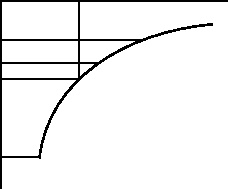
\includegraphics[width=0.28\textwidth]{gesamttex/edit_VIII-4/images/LH_37_03_125-127_d3_126v.pdf}%
\edcaption[-1.00em]%
{%
\hspace{1.50mm}\lbrack\textit{Fig.\:3}\rbrack%
}%
\end{edfigure}%
\pstart%
(16)
Ut vero generaliter praedicere possimus
dato pondere%
\indexS{pondus comprimens aerem}
quantum futurum sit spatium,%
\indexS{spatium intra quod aer comprimitur}
manifestum est ex dictis
tres rectas:
\edtext{%
altitudinem aeris compressi,%
\indexS{altitudo aeris compressi}
ut \textit{AH},
rectam \textit{DE}
et denique altitudinem%
\indexS{altitudo liquidi comprimentis}%
}{%
\lemma{altitudinem}%
\Bfootnote{%
\textit{(1)}~spatii %
\textit{(2)}~ut \textit{AH} in %
\textit{(3)}~aeris compressi, ut \textit{AH}, %
\textit{(a)}~altitud %
\textit{(b)}~rectam \textit{DE} et denique %
\textit{(aa)}~pondus %
\textit{(bb)}~altitudinem%
~\textit{L}%
}}
liquidi comprimentis \textit{HG},%
\indexS{liquidum comprimens}
esse continue proportionales,%
\indexS{proportio continua}
adeoque quadratum ipsius \textit{DE}%
\indexS{quadratum aequale rectangulo}
divisum per ipsam \textit{AH}
\edtext{%
dare
\lbrack\textit{HG}\rbrack,
et idem divisum per
\lbrack\textit{HG}\rbrack\
dare \textit{AH}.
Imo etsi ignoremus rectam \textit{DE},
sufficiet
unum experimentum in tubo fecisse%
\indexS{experimentum in tubo}%
\indexS{tubus plenus aere}
ad praedicendum eventum%
\indexS{eventus praedicendus}
reliquorum.%
}{%
\lemma{dare}%
\Bfootnote{%
\bars{\textit{AG} \textit{ändert Hrsg.}} %
et idem divisum per %
\bars{\textit{AG} \textit{ändert Hrsg.}} %
dare \textit{AH} %
\textit{(1)}~, idque procedet %
\textit{(2)}~. Imo etsi %
\lbrack...\rbrack\ eventum reliquorum.%
~\textit{L}%
}}
Si enim experimentum%
\indexS{experimentum in tubo}
sub signo%
\indexS{signum}
\astrosun\ fecerimus %
\edtext{%
modo dicto in artic.\;praecedente,%
\indexS{articulus}%
}{%
\lemma{modo \lbrack...\rbrack\ praecedente}%
\Cfootnote{%
\refpassage{LH_37_03_125-127_126v_wdrf-1}{LH_37_03_125-127_126v_wdrf-2}.%
}}
et rectang. \textit{ANM}%
\indexS{rectangulum}
dividerimus per datum pondus \textit{HG},%
\indexS{pondus comprimens aerem}
habebimus quaesitum spatium aeris \textit{AH};%
\indexS{spatium intra quod aer comprimitur}
sin idem rectangulum%
\indexS{rectangulum}
dividamus per datum spatium \textit{AH},%
\indexS{spatium intra quod aer comprimitur}
\edtext{%
habebimus \textit{HG} quaesitam altitudinem ponderis%
\indexS{altitudo ponderis quaesita}%
}{%
\lemma{habebimus}%
\Bfootnote{%
\textit{(1)}~quaesitum pond %
\textit{(2)}~%
\bars{\textit{HG} \textit{erg.}} quaesitam altitudinem
\textit{(a)}~liquidi %
\textit{(b)}~ponderis%
~\textit{L}%
}}
aerem in datum spatium%
\indexS{spatium intra quod aer comprimitur}%
\indexS{pondus comprimens aerem}
\edtext{%
compressuri.
\lbrack%
\href{\Scan{LH_37_03_127r}}%
{127\:r\textsuperscript{o}}%
\rbrack\
Quodsi altitudines istae non sint datae in numeris,%
\indexS{altitudo aeris compressi}%
\indexS{altitudo ponderis comprimentis}%
\indexS{altitudo liquidi comprimentis}
sed tantummodo in lineis,
semper tamen Geometrice praestari poterit quaesitum%
\indexS{quaesitum geometrice praestitum}
per inventionem quartae proportionalis,%
\indexS{inventio quartae proportionalis}%
\indexS{quarta proportionalis}%
}{%
\lemma{compressuri.}%
\Bfootnote{%
\textit{(1)}~Quodsi %
\textit{(a)}~\textlangle lineae\textrangle\ %
\textit{(b)}~altitudines %
\textit{(c)}~altitudines non sint datae %
\bars{\textlangle in num\textrangle eris \textit{gestr.}}, semper tamen res ad tertiae vel quartae %
\lbrack\href{\Scan{LH_37_03_127r}}{127\:r\textsuperscript{o}}\rbrack\ %
\textit{(2)}~Quodsi altitudines %
\bars{istae \textit{erg.}} non sint datae in %
\textit{(a)}~lineis sed tantum in %
\textit{(aa)}~\textlangle inn\textrangle\ %
\textit{(bb)}~in %
\textit{(b)}~numeris, sed %
\lbrack...\rbrack\ quartae proportionalis,%
~\textit{L}%
}}
quia ut \textit{AH} ad \textit{AN} %
ita \textit{NM} ad \textit{HG},
\edtext{%
\textls{per artic.\;14.}%
}{%
\lemma{per artic.\;14}%
\Cfootnote{%
\refpassage{LH_37_03_125-127_126v_zcvyj-1}{LH_37_03_125-127_126v_zcvyj-2}.%
}}%
\pend%
\newpage%
\pstart%
\edlabel{LH_37_03_125-127_127rv_progrharmon-1}%
(17)
Ut autem naturam%
\indexS{natura progressionis}
\edtext{%
Progressionis
secundum quam
aucto pondere%
\indexS{pondus comprimens aerem}
spatium minuitur%
\indexS{spatium intra quod aer comprimitur}%
\lbrack,\rbrack\
penitus explicem,%
}{%
\lemma{Progressionis}%
\Bfootnote{%
\textit{(1)}~hujus penitus explicem, %
\textit{(2)}~secundum quam %
\lbrack...\rbrack\ penitus explicem,%
~\textit{L}%
}}
prius hoc lemma demonstrandum est:%
\indexS{lemma demonstrandum}%
\textls{ }%
\edlabel{LH_37_03_125-127_127r_ext-1}%
\textls{Si sint quantitates quotcunque in progressione
\indexS{progressio arithmetica}%
Arithmetica,}
ut \textit{DE}, \textit{GE}, \textit{KE} etc.,%
\textls{ sintque aliae }%
\edtext{%
\textls{totidem }%
\textit{AF}, \textit{AH}, \textit{AL} etc.%
}{%
\lemma{\textls{totidem}}%
\Bfootnote{%
\textit{(1)}~\textlangle\textendash\textrangle\ %
\textit{(2)}~\textit{AG} %
\textit{(3)}~\textit{AF}, \textit{AH}, \textit{AL} etc.%
~\textit{L}%
}}%
\textls{ quae sint prioribus reciproce proportionales }%
(id
\edtext{%
est,
\edlabel{LH_37_03_125-127_127r_ve8c-1}%
sit \textit{DE} ad \textit{GE} ut $AH : AF,$
itemque
\textit{DE} ad \textit{KE} ut $AL : AF$%
\edlabel{LH_37_03_125-127_127r_ve8c-2}
etc.,
unde et \textit{GE} ad \textit{KE} ut \textit{AL} ad \textit{AH} etc.)%
}{%
\lemma{est,}%
\Bfootnote{%
\textit{(1)}~ut %
\textit{(a)}~\textit{DE}~: %
\textit{(b)}~$DE : KE$ %
\textit{(2)}~sit \textit{DE} ad %
\lbrack...\rbrack\ ut $AL : AF$ %
\textit{(a)}~etc.) %
\textit{(b)}~\textlangle et\textrangle\ $GE : KE \squaredots AL : AH$ etc.) %
\textit{(c)}~etc., unde %
\lbrack...\rbrack\ ad \textit{AH} etc.)%
~\textit{L}%
}}%
\textls{ tunc ipsas }%
\edtext{%
\textit{AF}, \textit{AH}, \textit{AL} etc.%
\textls{ fore}%
}{%
\lemma{\textit{AF}, \textit{AH}, \textit{AL}}%
\Bfootnote{%
\textit{(1)}~fore %
\textit{(2)}~etc. \textls{fore}~%
~\textit{L}%
}}%
\textls{ progressionis }%
\indexS{progressio harmonica}%
\edtext{%
\textls{Harmonicae }%
\edlabel{LH_37_03_125-127_127r_drzh-1}%
seu fore $AF - AH$ ad $AH - AL$
ut \textit{AF} ad \textit{AL}.%
\edlabel{LH_37_03_125-127_127r_ext-2}%
}{%
\lemma{\textls{Harmonicae}}%
\Bfootnote{%
\textit{(1)}~. Sit \textit{DE} aequ. \textit{x} %
\textit{(2)}~. Sit \textit{DE} aequ. %
\textit{(3)}~seu %
\textit{(a)}~erit %
\textit{(b)}~fore $AF - AH$ %
\lbrack...\rbrack\ \textit{AF} ad \textit{AL}.%
~\textit{L}%
}}
Cum enim sit \textit{GE} ad \textit{DE} ut \textit{AF} ad \textit{AH},
erit dividendo $GE - DE$ ad \textit{DE} ut $AF - AH$
\edtext{%
ad \textit{AH}.
Ergo rectangulum sub $GE - DE$ et \textit{AH}
aequale rectangulo sub \textit{DE} et $AF - AH.$%
\indexS{rectangulum}
Similiter,
quia \textit{KE} ad \textit{GE} ut \textit{AH} ad~\textit{AL},
erit dividendo $KE - GE$ ad \textit{GE} ut $AH - AL$ ad \textit{AL},
et rectang. sub $KE -GE$ et \textit{AL} aequale rectangulo sub \textit{GE} et $AH - AL.$
Ergo rectang. sub \textit{DE} et $AF - AH$ est ad rectang. sub \textit{GE} et $AH - AL$
ut rectang. sub $GE - DE$ et \textit{AH} ad rectang. sub $KE - GE$ et \textit{AL},
id est ut \textit{AH} ad \textit{AL},
demta communi altitudine
$GE - DE$ aequal. $KE - GE.$
Nam $GE - DE$ aequal. $KE - GE$
ob naturam progressionis Arithmeticae,%
\indexS{progressio arithmetica}%
\indexS{natura progressionis}
ubi semper differentiae terminorum quorumcunque%
\indexS{termini progressionis proximi}%
\indexS{differentia terminorum proximorum}
sibi proximorum sunt aequales.
Quoniam ergo rectang. sub \textit{DE} et $AF - AH$
est ad rectang. sub \textit{GE} et $AH - AL$%
\indexS{rectangulum}
ut \textit{AH} ad \textit{AL},
erit ratio \textit{AH} ad \textit{AL}
composita ex rationibus%
\indexS{ratio composita e rationibus}
\textit{DE} ad \textit{GE} et $AF - AH$ ad $AH- AL.$
Ergo vicissim%
}{%
\lemma{ad \textit{AH}.}%
\Bfootnote{%
\textit{(1)}~%
\bars{Jam rectang. sub $GE - DE$ et \textit{AH} aequal. rectangulo sub \textit{DE} et $AF- AH$ \textit{erg. u. gestr.}}
Similiter, quia \textit{KE} ad \textit{GE} ut \textit{AH} ad \textit{AL}, erit dividendo $KE - GE$ ad \textit{GE} ut $AH - AL$ ad \textit{AL}.
\bars{Ergo ratio composita ex ratione $GE - DE$ ad $KE - GE$ et ex ratione \textit{GE} ad \textit{DE} est eadem cum ratione composita \textit{erg. u. gestr.}}
Est autem $GE - DE$ aequal. $KE - GE$ (ex natura progressionis arithmeticae ubi differentiae terminorum duorum %
\textit{(a)}~vicinorum %
\textit{(b)}~proximorum sunt aequales) %
\textit{(2)}~Ergo rectangulum sub $GE - DE$ et \textit{AH} %
\textit{(a)}~et sub \textit{DE} %
\textit{(b)}~aequale rectangulo %
\lbrack...\rbrack\ et $AH - AL.$ Ergo %
\textit{(aa)}~rectang. sub $GE - DE$ et \textit{AH} est ad %
\textit{(bb)}~rectang. sub %
\lbrack...\rbrack\ $KE - GE$ et \textit{AL},
\textit{(aaa)}~(id est q %
\textit{(bbb)}~id est ut %
\textit{(ccc)}~id est %
\lbrack...\rbrack\ altitudine $GE - DE$ aequal. $KE - GE$ %
\textit{(aaaa)}~(quia %
\textit{(bbbb)}~. Nam $GE - DE$ aequal. $KE - GE$ %
\bars{( \textit{gestr.}} ob naturam %
\lbrack...\rbrack\ sunt aequales. %
\bars{) \textit{gestr.}} Quoniam ergo %
\lbrack...\rbrack\ $AF - AH$ ad $AH- AL$
\textit{(aaaaa)}~adeoque vicissim %
\textit{(bbbbb)}~. Ergo vicissim%
~\textit{L}%
}}
ratio $AF - AH$ ad $AH - AL$
composita est ex%
\indexS{ratio composita e rationibus}
\edtext{%
rationibus \textit{GE} ad \textit{DE} et \textit{AH} ad~\textit{AL}.%
}{%
\lemma{rationibus}%
\Bfootnote{%
\textit{(1)}~\textit{AH} %
\textit{(a)}~ad \textit{AL} et %
\textit{(b)}~et %
\textit{(2)}~\textit{GE} ad %
\lbrack...\rbrack\ ad \textit{AL}.%
~\textit{L}%
}}
Jam ratio \textit{GE} ad \textit{DE} eadem est
cum ratione \textit{AF}
\edtext{%
ad \textit{AH}
(per
\edtext{%
dicta sub initium huius demonstrationis).%
\indexS{demonstratio}%
}{%
\lemma{dicta \lbrack...\rbrack\ demonstrationis}%
\Cfootnote{%
Vgl. \refpassage{LH_37_03_125-127_127r_ve8c-1}{LH_37_03_125-127_127r_ve8c-2}.%
}}%
}{%
\lemma{ad \textit{AH}}%
\Bfootnote{%
\textit{(1)}~(ob %
\textit{(a)}~\textit{DE} %
\textit{(b)}~\textit{GE}, \textit{DE} et \textit{AH} ad \textit{AF} recipro %
\textit{(2)}~(per %
\textit{(a)}~superiora %
\textit{(b)}~dicta sub initium huius demonstrationis).%
~\textit{L}%
}}
Ergo
\edtext{%
ratio
$AF - AH$ ad $AH - AL$
composita est ex rationibus%
\indexS{ratio composita e rationibus}
\textit{AF} ad \textit{AH} et \textit{AH} ad \textit{AL},%
}{%
\lemma{ratio}%
\Bfootnote{%
\textit{(1)}~\textit{AF} ad %
\textit{(2)}~$AF - AH$ ad %
\lbrack...\rbrack\ ex rationibus %
\textit{(a)}~\textit{AH} ad %
\textit{(b)}~\textit{AF} ad %
\lbrack...\rbrack\ ad \textit{AL},%
~\textit{L}%
}}
quae eadem est cum ratione \textit{AF} ad \textit{AL}.
Ergo $AF - AH$ est ad $AH - AL$ ut \textit{AF} ad \textit{AL}.
Seu termini extremi \textit{AF} et \textit{AL}%
\indexS{termini proportionis extremi}
sunt inter se
ut $AF - AH$ et $AH - AL$
\edtext{%
\textlangle seu u\textrangle t%
}{%
\lemma{\textlangle seu u\textrangle t}%
\Cfootnote{%
Beide Worte noch lesbar in dem 1967 aufgenommenen S-Film Nr. 116 der GWLB Hannover.%
}}
differentiae extremorum a%
\indexS{differentia terminorum extremorum a medio}
\edtext{%
medio \textit{AH}.%
\indexS{terminus proportionis medius}
Ergo%
}{%
\lemma{medio \textit{AH}.}%
\Bfootnote{%
\textit{(1)}~Adeoque %
\textit{(2)}~Ergo%
~\textit{L}%
}}
hi tres termini
\edtext{\textit{AF}, \textit{AH}, \textit{AL}%
}{%
\lemma{\textit{AF}, \textit{AH}, \textit{AL}}%
\Bfootnote{%
\textit{erg.\;L}%
}}
sunt progressionis harmonicae.%
\indexS{progressio harmonica}%
\edlabel{LH_37_03_125-127_127r_drzh-2}
\lbrack%
\href{\Scan{LH_37_03_127v}}%
{127\:v\textsuperscript{o}}%
\rbrack\
Idemque patet
de tribus aliis continuis quibuscunque,%
\indexS{termini proportionis continuae}
si
\edtext{%
plures tribus secundum%
}{%
\lemma{plures}%
\Bfootnote{%
\bars{tribus \textit{erg.}} secundum%
~\textit{L}%
}}
\edtext{%
conditiones%
\indexS{conditio}
\edtext{%
initio hujus articuli%
\indexS{articulus}
dictas%
}{%
\lemma{initio}%
\Bfootnote{%
\textit{(1)}~dictas %
\textit{(2)}~hujus articuli dictas%
~\textit{L}%
}}%
}{%
\lemma{conditiones \lbrack...\rbrack\ dictas}%
\Cfootnote{%
\refpassage{LH_37_03_125-127_127r_ext-1}{LH_37_03_125-127_127r_ext-2}.%
}}
assumantur%
\lbrack;\rbrack\
adeoque
\edtext{%
tota series quotcunque%
}{%
\lemma{tota}%
\Bfootnote{%
\textit{(1)}~quotcunque %
\textit{(2)}~series quotcunque%
~\textit{L}%
}}
terminorum hujusmodi
\textit{AF}, \textit{AH}, \textit{AL} etc.
progressionis harmonicae erit.%
\indexS{progressio harmonica}
Q.E.D.%
\edlabel{LH_37_03_125-127_127rv_progrharmon-2}
\pend%
\pstart%
(18)
Hinc sequitur%
\textls{ fractiones quaecunque,%
\indexS{fractio reciproce proportionalis numeratori}
quorum numerator sit idem,%
\indexS{numerator fractionis}
nominatores%
\indexS{nominator fractionis}
vero }%
\edtext{%
\textls{sint progressionis arithmeticae,%
\indexS{progressio arithmetica}
fore progressionis harmonicae}%
\indexS{progressio harmonica}%
}{%
\lemma{\textls{sint progressionis}}%
\Bfootnote{%
\textit{(1)}~harmonicae, fore prog %
\textit{(2)}~\textls{arithmeticae, fore progressionis harmonicae}%
~\textit{L}%
}}%
\textls{ }%
ut
\rule[-2,8mm]{0mm}{6.9mm}%
$\displaystyle\frac{1}{1}\,~\frac{1}{2}\,~\frac{1}{3}\,~\frac{1}{4}\,~\frac{1}{5}$ etc.
Sunt enim hae fractiones reciproce proportionales%
\indexS{fractio reciproce proportionalis numeratori}
\edtext{%
suis nominatoribus,%
\indexS{nominator fractionis}
ac proinde%
}{%
\lemma{}%
\Bfootnote{%
suis nominatoribus, ac proinde
\textit{erg.\;L}%
}}
totidem numeris progressionis Arithmeticae,%
\indexS{progressio arithmetica}
nempe
\edtext{%
1\,~2\,~3\,~4\,~5.
Est enim%
\rule[-2mm]{0mm}{0mm}
\newline%
\hspace*{7.5mm}%
$\displaystyle\frac{1}{1}$ ad $\displaystyle\frac{1}{2}$ ut 2 ad 1,%
\rule[-4mm]{0mm}{8mm}
\newline%
\hspace*{7.5mm}%
$\displaystyle\frac{1}{1}$ ad $\displaystyle\frac{1}{3}$ ut 3 ad 1,%
\rule[-4mm]{0mm}{8mm}
\newline%
\hspace*{7.5mm}%
$\displaystyle\frac{1}{1}$ ad $\displaystyle\frac{1}{4}$ ut 4 ad 1,%
\rule[-4mm]{0mm}{8mm}
\newline%
\hspace*{7.5mm}%
$\displaystyle\frac{1}{2}$ ad $\displaystyle\frac{1}{3}$ ut 3 ad 2,%
\rule[-4mm]{0mm}{8mm}
\newline%
\hspace*{7.5mm}%
etc.
\newline%
Jam%
\edtext{%
\textls{ per artic.\;praecedentem }%
}{%
\lemma{\textls{per artic.\;praecedentem}}%
\Cfootnote{%
ebd.%
}}%
termini quotcunque totidem arithmeticis%
\indexS{termini arithmetici}
reciproce proportionales%
\indexS{termini reciproce proportionales terminis arithmeticis}
sunt progressionis harmonicae.%
\indexS{progressio harmonica}
Ergo hae fractiones sunt progressionis harmonicae.%
\indexS{progressio harmonica}%
}{%
\lemma{1~2~3~4~5.}%
\Bfootnote{%
\textit{(1)}~Ergo \textls{per artic. praecedentem ipsae fractiones sunt progressionis harmonicae.} %
\textit{(2)}~Est enim %
\lbrack...\rbrack\ progressionis harmonicae.%
~\textit{L}%
}}
\pend%
\newpage%
\pstart%
\noindent%
\lbrack\textit{Auf der rechten Spalte von Bl.~\href{\Scan{LH_37_03_127r}}{127\:r\textsuperscript{o}} als Nebenrechnung zum Abschnitt Nr.} 17 \textit{(\refpassage{LH_37_03_125-127_127r_drzh-1}{LH_37_03_125-127_127r_drzh-2})%
}:\rbrack\
\pend%
\vspace{2.0em}%
\pstart%
$%
\displaystyle%
\efrac{AF}{x}
\quad\quad\quad \ \ %
\efrac{AH}{y}
\quad\quad\quad \ \ \ %
\efrac{AL}{z}%
$%
\pend%
\vspace{1.5em}%
\pstart%
$%
\displaystyle%
\efrac{\displaystyle\frac{a^2}{a}}{\rule[0mm]{0mm}{4mm}DE}
\quad\quad%
\efrac{\displaystyle\frac{a^2}{a + d \sqcap b}}{\rule[0mm]{0mm}{4mm}GE}
\quad\quad%
\efrac{\displaystyle\frac{a^2}{a + 2d \sqcap c}}{\rule[0mm]{0mm}{4mm}KE}%
$%
\edlabel{LH_37_03_125-127_127r_akn-1}%
\edtext{}{%
\xxref{LH_37_03_125-127_127r_akn-1}{LH_37_03_125-127_127r_akn-2}%
\lemma{\textit{KE}}%
\Bfootnote{%
\textit{(1)}~\lbrack/\rbrack\ $\displaystyle\frac{x}{y} \sqcap \frac{a + d}{a}.$ %
\textit{(2)}~\lbrack/\rbrack\ $\displaystyle\frac{a + d}{a} \sqcap \frac{x}{y}.$
\textit{(3)}~$\displaystyle\efrac{a + d}{}$
\textit{(4)}~\lbrack/\rbrack\ $\displaystyle\frac{a}{a + d} \sqcap \frac{y}{x}.$%
~\textit{L}%
}}%
\pend%
\vspace{1.75em}%
\pstart%
$%
\displaystyle%
\frac{a}{a + d} \sqcap \frac{y}{x}.%
\edlabel{LH_37_03_125-127_127r_akn-2}%
$%
\pend%
\vspace{1.75em}%
\pstart%
$%
\displaystyle%
\frac{b}{a} \sqcap \frac{x}{y}.
\quad\quad\quad%
\frac{c}{a} \sqcap
\edtext{%
\lbrack\frac{x}{z}\rbrack.%
}{%
\lemma{$\displaystyle\frac{z}{x}$}%
\Bfootnote{%
\textit{L~ändert Hrsg.}%
}}
\quad\quad\quad%
\frac{c}{b} \sqcap \frac{y}{z}.
$%
\pend%
\vspace{1.75em}%
\pstart%
$%
\displaystyle%
\frac{x - y}{y} \sqcap \frac{b - a}{a}
\quad\quad\quad%
\frac{y - z}{z} \sqcap \frac{c - b}{b}.%
$%
\edlabel{LH_37_03_125-127_127r_vhb-1}%
\edtext{}{%
\xxref{LH_37_03_125-127_127r_vhb-1}{LH_37_03_125-127_127r_vhb-2}%
\lemma{$\displaystyle\frac{c - b}{b}.$\rule[0mm]{0mm}{5mm}}%
\Bfootnote{%
\textit{(1)}~\lbrack/\rbrack\ $\displaystyle\frac{x - y}{y - z} \sqcap \frac{y}{z}$ %
\textit{(2)}~$\displaystyle\frac{x - y}{y - z} \sqcap \efrac{b - a}{}$ %
\textit{(3)}~\lbrack/\rbrack\ $\displaystyle\frac{x - y}{y - z} \smallfrown $ %
\textit{(a)}~$\displaystyle\frac{y}{z}$ %
\textit{(b)}~$\displaystyle\frac{z}{y} \ \text{aequ.} \ \frac{b - a}{c - b} \smallfrown \frac{b}{a}.$%
~\textit{L}%
}}%
\pend%
\vspace{1.75em}%
\pstart%
$%
\displaystyle%
\frac{x - y}{y - z} \smallfrown \frac{z}{y}
\ \text{aequ.} \
\frac{b - a}{c - b} \smallfrown \frac{b}{a}.
$%
\edlabel{LH_37_03_125-127_127r_vhb-2}%
\pend%
\vspace{1.75em}%
\pstart%
Est autem
$%
\displaystyle%
b - a \ \text{aequ.} \ c - b.
$%
\pend%
\vspace{1.75em}%
\pstart%
Ergo
$%
\displaystyle%
\frac{x - y}{y - z} \smallfrown \frac{z}{y}
\ \text{aequ.} \
\frac{b}{a}.
$%
\pend%
\vspace{1.75em}%
\pstart%
Ergo
$%
\displaystyle%
\frac{x - y}{y - z} \sqcap \frac{b}{a} \smallfrown \frac{y}{z} \sqcap \frac{x}{y} \smallfrown \frac{y}{z} \sqcap \frac{x}{z}.
$%
\pend%
\newpage%
\newpage%
\vspace{3.0em}%
\pstart%
\noindent%
\centering%
*     *     *
\pend%
\vspace{2.5em}%
\selectlanguage{latin}%
\frenchspacing%
\begin{ledgroup}%
\footnotesize%
\pstart%
\noindent%
\textls{Ausführliche Datierungsgründe:}%
\pagelabel{60212_dat}
In der undatierten und titellosen Aufzeichnung N.\;\ref{60212} befasst sich Leibniz ausführlich mit dem elastischen Verhalten einer Luftmasse, die in einem geschlossenen Raum zusammengedruckt wird.
Im Mittelpunkt der Untersuchung steht das Verhältnis zwischen dem Volumen der Luftmasse und dem Druck, den eine aufgesetzte Quecksilbermasse übt.
Eine direkte Berechnung der elastischen Kraft wird nicht unternommen.
Vielmehr wird festgestellt, dass die "elastische Kraft" (\textit{elastrum}), mit der die zusammengedruckte Luftmasse sich zu befreien dränge, proportional zur "druckenden Kraft" (\textit{vis comprimens}), d.\,h. zum Gewicht der Quecksilbermasse, wachse, während das Volumen der Luftmasse sich umgekehrt proportional verringere; siehe vornehmlich die Abschnitte Nr.\;(10) und Nr.\;(12) im Text.
\pend%
\pstart%
Das im Träger der Aufzeichnung N.\;\ref{60212} anzutreffende Wasserzeichen (eine achtblättrige Rosette über den Buchstaben CS; vgl. Bl.\:\href{\Scan{LH_37_03_125wz}}{125}) ist im Leibniz-Nachlass für die ersten Hannoveraner Jahre (etwa bis 1685) häufig belegt.
Inhaltliche Gründe für eine Einschränkung der Datierung liefert der Vergleich mit den Briefen, die Leibniz zwischen August und September 1679 mit dem Kieler Juristen und Mathematiker Samuel Reyher\indexN{\textls{Reyher} (Reiherus, Reiher), Samuel 1635\textendash1714} austauschte.
In seinem Schreiben vom 24\; (3.\;September) 1679 bedankt sich Reyher für den Vorschlag einer \textit{divisio thermometri}, den ihm Leibniz am 12.\;(22.) August 1679 mitgeteilt hat, äußert aber Zweifel an Leibnizens Behauptung, die Einteilung der thermometrischen Skala solle nach harmonischer Progression erfolgen (\textit{LSB} III,\;2 N.\;333, S.\;808.16\,f.;\cite{01436}
N.\;338, S.\;823.11--16).\cite{01434}
Reyher bemerkt zudem, der Zweifel lasse sich wohl durch ein \textit{experimentum per pondera corpori elastico imponenda} klären (\textit{LSB} III,\;2 N.\;338 S.\;823.16\,f.).\cite{01434}
Auf diese Andeutung geht Leibniz ausdrücklich in seiner Antwort vom 8.\;September 1679 ein, indem er ein Gedankenexperiment entwirft, das in erheblichem Maße demjenigen ähnelt, das im Mittelpunkt der vorliegenden Aufzeichnung N.\;\ref{60212} steht:
Wenn in einem im Vakuum stehenden Rohr eine Quecksilbermasse eine eingekesselte Luftmasse zusammendrücke, dann ergebe sich bei einer linearen Gewichtszunahme der Quecksilbermasse, dass der von der Luft eingenommene Raum nach harmonischer Progression abnehme, d.\,h. in umgekehrter Proportionalität (\textit{LSB} III,\;2 N.\;341, S.\;828.9--829.15).\cite{01435}
Zu demselben Ergebnis kommt Leibniz auch in N.\;\ref{60212} (bes. \refpassage{LH_37_03_125-127_127rv_progrharmon-1}{LH_37_03_125-127_127rv_progrharmon-2};
vgl. zudem das Diagramm \lbrack\textit{Fig.\:2}\rbrack\ in N.\;\ref{60212} mit der Abbildung in \textit{LSB} III,\;2 N.\;341, S.\;828).\cite{01435}
Das Ergebnis dieses Gedankenexperiments kennzeichnet Leibniz in seiner Antwort auf Reyher als empirisch (\textit{quemadmodum tentando comperies}); er kündigt jedoch an, der entsprechende Beweis sei bereits in Vorbereitung (\textit{Quanquam et demostratio in promtu sit}; \textit{LSB} III,\;2 N.\;341, S.\;829.13).\cite{01435}
Die Vermutung liegt somit nahe, dass Leibnizens Ankündigung auf die vorliegende Aufzeichnung N.\;\ref{60212} anspielt.
Unter dieser Voraussetzung ist anzunehmen, dass sie in engem zeitlichem Zusammenhang mit Leibnizens Antwort an Reyher\indexN{\textls{Reyher} (Reiherus, Reiher), Samuel 1635\textendash1714} entstand, d.h. wohl noch im September 1679.
\pend%
\pstart%
Eine spätere Abfassungszeit der Aufzeichnung N.\;\ref{60212} ist unwahrscheinlich, aber nicht auszuschließen.
Die Texte
\textit{LSB} VIII,\;3 N.\;14\textsubscript{3} (Januar -- März/April 1683),\cite{01437}
N.\;14\textsubscript{7} (März/April 1683 -- erste Hälfte 1684),\cite{01438}
N.\;17 (Ende Januar 1683 -- Ende 1684)\cite{01439}
und N.\;21 (Ende Januar 1683 [?] -- Juli 1686 [?])\cite{01440}
setzen jedoch mutmaßlich die Ergebnisse von N.\;\ref{60212} voraus.
Wenn diese Vermutung zutrifft, dann ist die vorliegende Aufzeichnung spätestens in den ersten Monaten 1683 entstanden.
\pend%
\pstart%
Abschließend gilt es zu bemerken, dass sämtliche Verweise auf die Aufzeichnung N.\;\ref{60212}, die in den Texten  \textit{LSB} VIII,\,3 N.\;14\textsubscript{3}\cite{01437} \textit{Explicatio mechanica elastri}, N.\;14\textsubscript{7}\cite{01438} \textit{Demonstratio quod extensiones elasticorum sint viribus tendentibus proportionales}, N.\;17\cite{01439} \textit{De viribus chordas ad rupturam tendendibus} und N.\;21\cite{01440} \textit{De vibrationibus aeris tensi}, sich als fraglich erwiesen haben.
Somit erweisen sich auch sämtliche von diesen Verweisen herrührenden Schlussfolgerungen als fraglich.
\pend%
\end{ledgroup}%
\selectlanguage{latin}%
\frenchspacing%
\normalsize%
\newpage%
